% Figure 2.5 (Session 2): the Abrikosov fermions, the bond operator and the spinon band.
% The image is rendered by figures/blender/s2_5_abrikosov.py; the coordinates of the labels
% come from figures/blender/out/abrikosov_anchors.tex. Compile with:
%   pdflatex abrikosov.tex ; result moves to ../quantum_magnetism/abrikosov.pdf
\documentclass[11pt,tikz,border=0pt]{standalone}
\usepackage{amsmath,amssymb,graphicx,braket,bm}\newcommand{\vb}[1]{\bm{#1}}
\usepackage{xcolor}
\definecolor{coursedark}{HTML}{1B2A4A}
\definecolor{costamber}{HTML}{B8620A}
\newlength{\figw}\setlength{\figw}{16.19cm}   % the text width of the notes (letter, 2.7 cm margins), so labels print at size
\newcommand{\up}{\uparrow}\newcommand{\dn}{\downarrow}

\begin{document}
\begin{tikzpicture}[lbl/.style={font=\small, text=coursedark}, gh/.style={font=\small, text=coursedark!45}]
  \node[anchor=south west, inner sep=0pt] at (0,0)
    {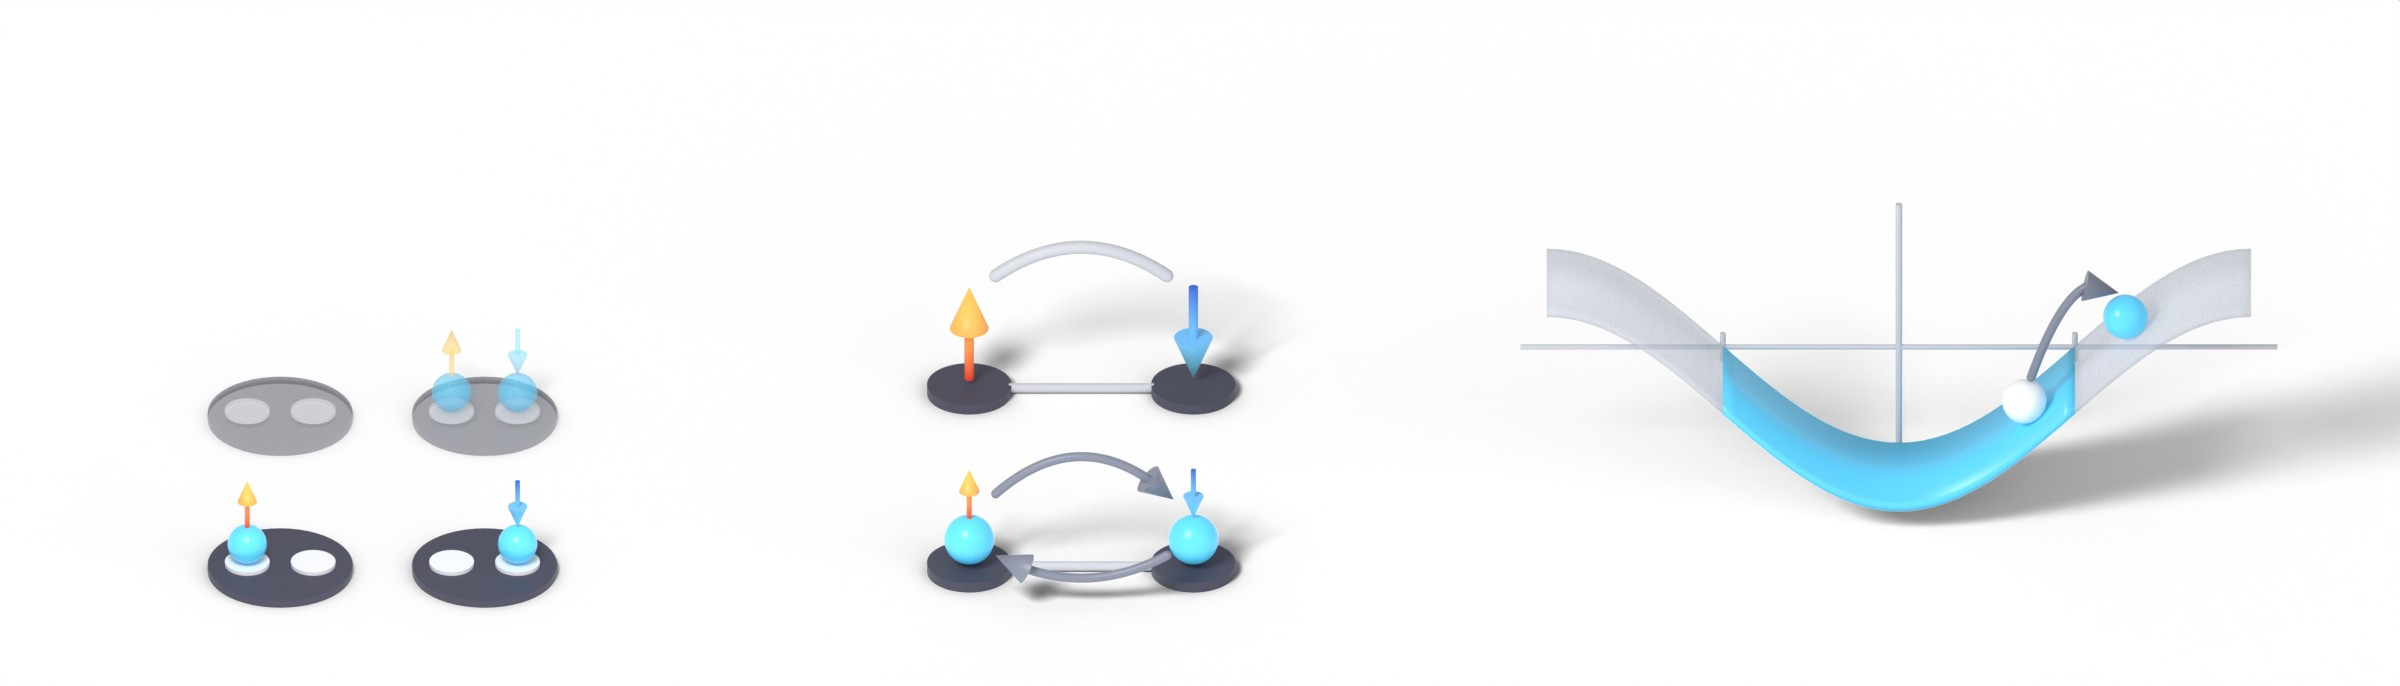
\includegraphics[width=\figw]{../blender/out/abrikosov.jpg}};
  %% written by figlib.py; x and y in units of the image width
\coordinate (k0) at (0.0783\figw,0.1157\figw);
\coordinate (k3) at (0.2404\figw,0.1157\figw);
\coordinate (k1) at (0.0783\figw,0.0525\figw);
\coordinate (k2) at (0.2404\figw,0.0525\figw);
\coordinate (a) at (0.0275\figw,0.2346\figw);
\coordinate (labA) at (0.1593\figw,0.0230\figw);
\coordinate (J) at (0.4505\figw,0.1899\figw);
\coordinate (chi) at (0.5220\figw,0.0729\figw);
\coordinate (b) at (0.3407\figw,0.2346\figw);
\coordinate (labB) at (0.4505\figw,0.0230\figw);
\coordinate (kF) at (0.8646\figw,0.1413\figw);
\coordinate (mkF) at (0.7178\figw,0.1413\figw);
\coordinate (eps) at (0.7912\figw,0.2008\figw);
\coordinate (kend) at (0.9489\figw,0.1413\figw);
\coordinate (c) at (0.6154\figw,0.2346\figw);
\coordinate (labC) at (0.7912\figw,0.0230\figw);

  \node[lbl, font=\normalsize, anchor=west] at (a) {(a)};
  \node[lbl, font=\normalsize, anchor=west] at (b) {(b)};
  \node[lbl, font=\normalsize, anchor=west] at (c) {(c)};
  \node[gh, anchor=east] at (k0) {$\ket{0}$};
  \node[gh, anchor=west] at (k3) {$\ket{\up\dn}$};
  \node[lbl, anchor=east] at (k1) {$\ket{\up}$};
  \node[lbl, anchor=west] at (k2) {$\ket{\dn}$};
  \node[lbl, anchor=north] at (labA) {$\sum_\sigma f^\dagger_{i\sigma}f_{i\sigma}=1$};
  \node[lbl, anchor=south] at (J) {$J\,\vb{S}_i\cdot\vb{S}_j$};
  \node[lbl, anchor=west] at (chi) {$\chi_{ij}^\dagger\chi_{ij}$};
  \node[lbl, anchor=north] at (labB) {the same bond, in fermions};
  \node[lbl, anchor=north west, inner sep=2pt] at (kF) {$k_F$};
  \node[lbl, anchor=north east, inner sep=2pt] at (mkF) {$-k_F$};
  \node[lbl, anchor=south] at (eps) {$\varepsilon(k)$};
  \node[lbl, anchor=west] at (kend) {$k$};
  \node[lbl, anchor=north] at (labC) {spinon band, filled up to $\pm k_F=\pm\pi/2$};
\end{tikzpicture}
\end{document}
